\documentclass[{../../master}]{subfiles}
\graphicspath{{../../}}  % 個別コンパイル時の画像パスを解決する

\begin{document}

\section{USBデバイスの接続}

ADAMR2では以下のUSBデバイスを使用します:

\begin{itemize}
  \item T-Frogモータードライバ(TF-2MD3-R6)
  \item RPLiDAR A2
  \item Intel Realsense D435
  \item Logicool F710 ゲームパッド(オプション)
\end{itemize}

他に,ディスプレイとしてHDMI接続のモバイルディスプレイを接続し,モバイルディスプレイとRPLiDARに5V電源を供給するためのモバイルバッテリーも搭載します.

各種デバイスの接続図を図\ref{fig:devices_connection}に示します.

\begin{figure}[ht]
  \centering
  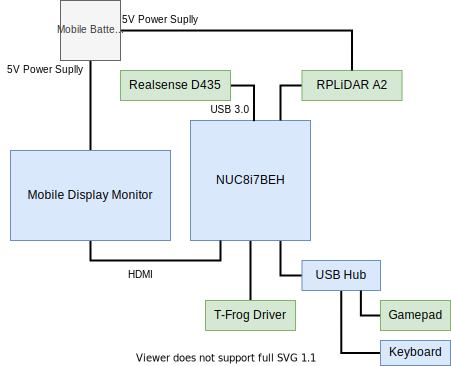
\includegraphics[]{images/devices_connection.drawio.pdf}
  \caption{USB Device Connection Diagram}
  \label{fig:devices_connection}
\end{figure}

注意点として,Intel Realsense D435とRPLiDAR A2は,USBハブを介した接続を行うと電流不足で動作しなくなる場合があります.
PCのUSBポートに直接接続し,電流不足を回避してください.
\footnote{RPLiDARは外部給電を行っているため電流不足にはならないはずなのですが,実際に電流不足に陥ることが多かったため,可能な限りPCのUSBポートに直接接続するようにしてください.}

\end{document}